\textit{Определение} \textbf{Основанные на энергии} подходы в машинном обучении представляют собой методы моделирования, основанные на понятии энергии системы $E$.

В этом подходе модель оценивает энергию данных, а затем использует эту оценку для различных задач, 
таких как классификация, регрессия или генерация данных.
 
Адаптация модели происходит через задачу оптимизации. В ходе градиентного спуска происходит поиск минимума энергии реальных данных.


Пусть \( \mathbf{x} \) — наблюдаемая переменная (например, вектор признаков),
 а \( E(\mathbf{x}; \theta) \) — энергия, присвоенная данным \( \mathbf{x} \) моделью с параметрами \( \theta \). 

Energy-based модели могут быть использованы для решения различных задач. Например, в задаче классификации модель может устанавливать низкую энергию для данных из правильного класса и высокую для данных из неправильного класса. Для регрессии модель может предсказывать энергию, близкую к целевому значению.

Обучение energy-based моделей часто включает минимизацию функции потерь, которая может быть определена как разница между энергией реальных данных и сгенерированных данных. Один из часто используемых подходов - это минимизация отклонения (discrepancy) между энергиями реальных данных \( \mathbf{x} \) и сгенерированных данных \( \tilde{\mathbf{x}} \):

\[ L(\theta) = E(\mathbf{x}; \theta) - E(\tilde{\mathbf{x}}; \theta) \]

Такой подход позволяет модели стремиться к минимизации энергии для реальных данных и максимизации энергии для сгенерированных данных.

Energy-based подходы имеют широкий спектр применений и используются в различных областях, включая глубокое обучение, генеративные модели и обучение без учителя. Они представляют собой мощный инструмент для моделирования данных с использованием концепции энергии, что позволяет справляться с различными задачами в машинном обучении.


\textit{Определение} \textbf{Диффузионные модели} \label{diffusion} представляют собой класс вероятностных моделей, 
использующих уравнение Ланжевена для генерации изображений.

\begin{figure}[h]
    \centering
    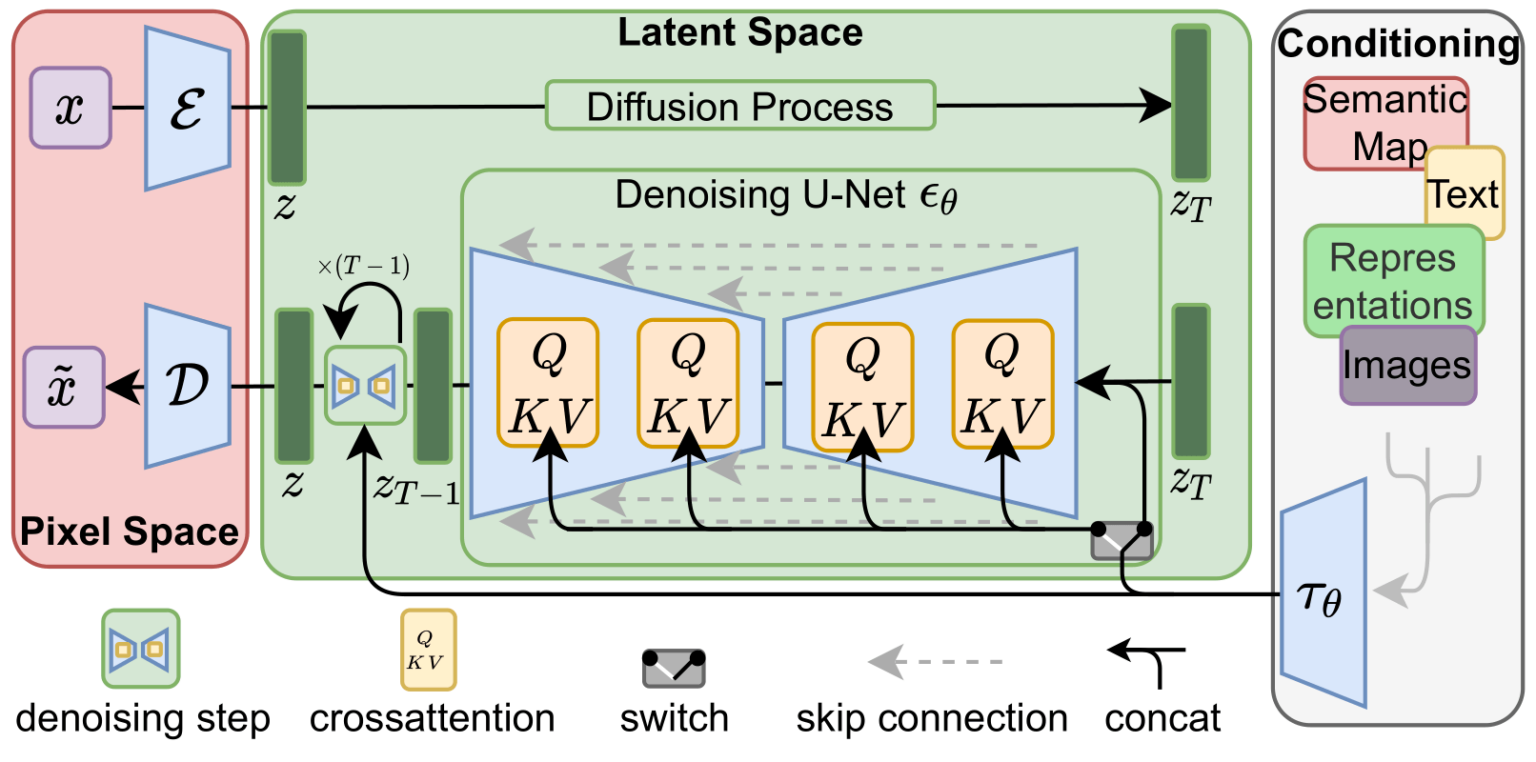
\includegraphics[width=0.5\textwidth]{assets/ml/generation/stable_diffusion.png}
    \caption{Иллюстрация модели Stable Diffusion \cite{stablediffusion}}
    \label{sd_arch}
\end{figure}

Обучение модели состоит из двух этапов.


\begin{figure}[h]
    \centering
    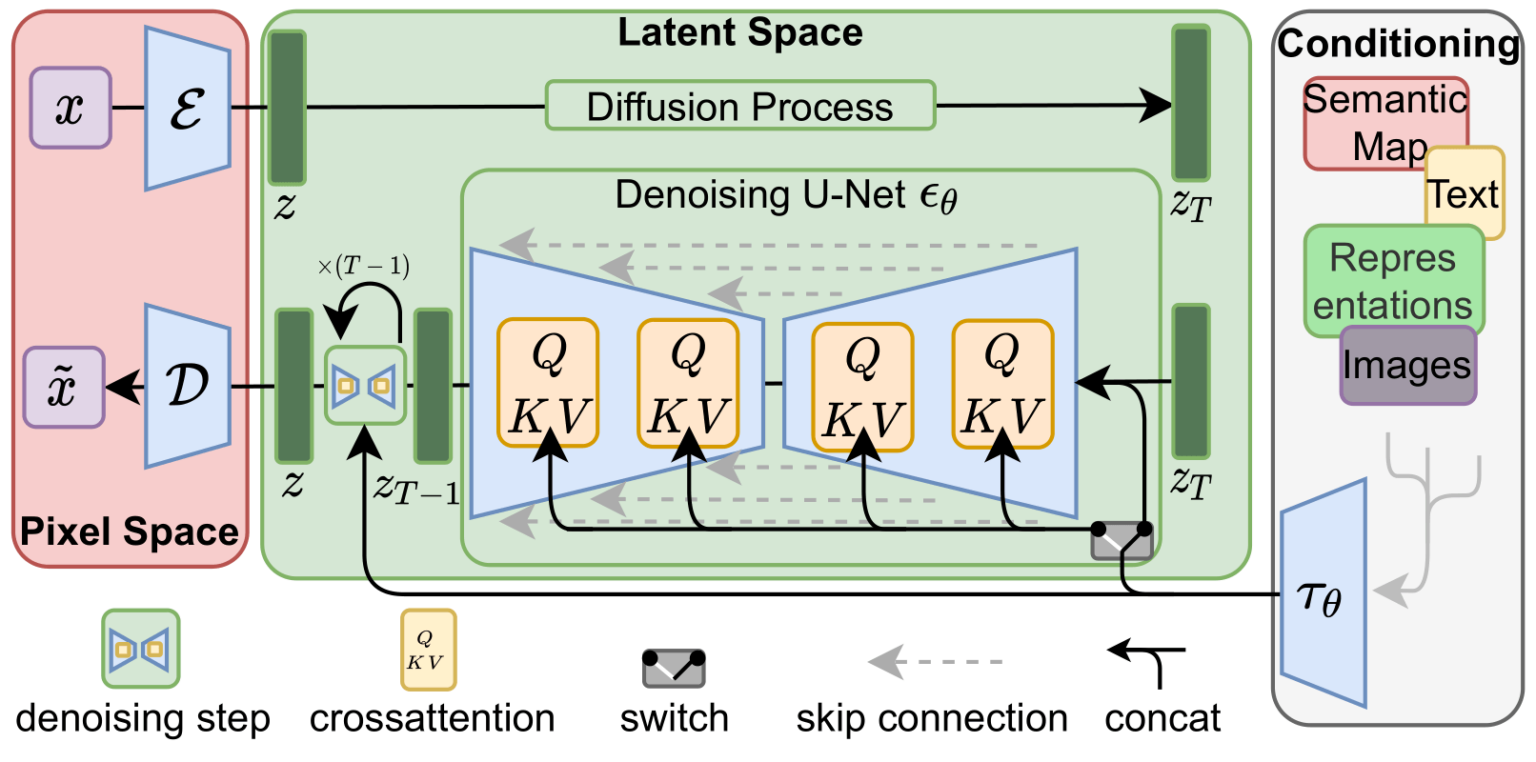
\includegraphics[width=0.5\textwidth]{assets/ml/generation/stable_diffusion.png}
    \caption{Иллюстрация модели Stable Diffusion \cite{stablediffusion}}
    \label{sd_learning}
\end{figure}

Обратный процесс.

- обучение нейронной сети для того,
 чтобы обратить процесс искажения вспять, то есть восстановить исходное изображение,
  синтезируя чистый шум путем постепенного снижения шума до тех пор, пока не будет получен чистый образец.



На практике функция ошибки без коэффициента 
имеет лучшие

$$
    \mathrm{E}_{x_0 \sim q; z\sim \mathcal{N}(0,I)} 
    \left[ \| \varepsilon_\theta(x_t,t) -z \|^2\right]
$$


Диффузионных модели выполняют генерация последовательными шагами, заключающимися 
в последовательном исправление ошибок из начального изображения.

Обучение исправлению ошибок выполняется путем 

$$
    \varepsilon \sim 
$$


Важным преимуществом диффузионных моделей является их способность генерировать высококачественные изображения без необходимости использования генеративно-состязательных сетей или других архитектур глубокого обучения. Кроме того, эти модели позволяют контролировать процесс генерации изображений, например, регулируя уровень шума или изменяя другие параметры.
Таким образом, диффузионные модели представляют собой эффективный и гибкий метод генерации изображений, который находит применение в различных областях, включая компьютерное зрение, графический дизайн и искусственный интеллект.

Обучение заключается в постепенном улучшение качество изображения путем приближения его к реальным данным из обучающего набора.



